
%\documentclass[10pt,twoside,twocolumn]{article}
\documentclass[12pt,twoside]{article}
\usepackage[bf,small]{caption}
\usepackage[letterpaper,hmargin=1in,vmargin=1in]{geometry}
\usepackage{paralist} % comapctitem, compactdesc, compactenum
\usepackage{titlesec}
\usepackage{titletoc}
\usepackage{times}
\usepackage{hyperref}
\usepackage{algorithmic}
\usepackage{graphicx}
\graphicspath{{./graphics/}}
\usepackage{xspace}
\usepackage{verbatim}
\usepackage{url}
\usepackage{float}
\hyphenation{Sub-Bytes Shift-Rows Mix-Col-umns Add-Round-Key}

\setlength{\parskip}{12pt}
\setlength{\parindent}{0pt}

\newcommand{\hdb}{\emph{hashdb}\xspace}
\newcommand{\bulk}{\emph{bulk\_extractor}\xspace}
\newcommand{\hashid}{\emph{hashid}\xspace}
\newcommand{\mdd}{\emph{md5deep}\xspace}
\newcommand{\bev}{\emph{Bulk Extractor Viewer}\xspace}

\begin{document}

\begin{center}
\Large Demo: Preparing a Block Hash Database \\
\large Using \mdd and \hdb
\end{center}

We build large databases of block hashes
to help us find matching blocks of data.
Here are some ways \hdb databases are used:
\begin{compactitem}
\item We scan data looking for blocks that match blocks in the blacklist databae.
\item We subtract whitelist blocks to remove distracting false positives.
\end{compactitem}
The Scanner demo at
\url{http://digitalcorpora.org/downloads/hashdb/demo/scanner\_demo.pdf}.
checks against a database of blacklisted hash values
to find part of a blacklisted video file in a media image.

The Similarity demo at
\url{http://digitalcorpora.org/downloads/hashdb/demo/similarity\_demo.pdf}.
subtracts whitelist hash values
to reveal blocks of user data that are common in two media images.

In this demo, we create a block hash database
for use as a blacklist or whitelist reference.
The workflow for managing blacklist databases and whitelist databases
is the same:
\begin{compactenum}
\item Generate DFXML file(s) of block hashes
from blacklist or whitelist file sources.
\item Import these DFXML file(s) into a block hash database.
\end{compactenum}

%Here is the workflow:
Generate block hashes in DFXML format:

\begin{figure}[H]
  \center
  
\includegraphics[scale=0.6]{drawings/md5deep}
  \caption*{Run \mdd to create a DFXML file of block hashes \\
            from your library of blacklist or whitelist files.}
\end{figure}

Import block hashes into the hash database:

\begin{figure}[H]
  \center
  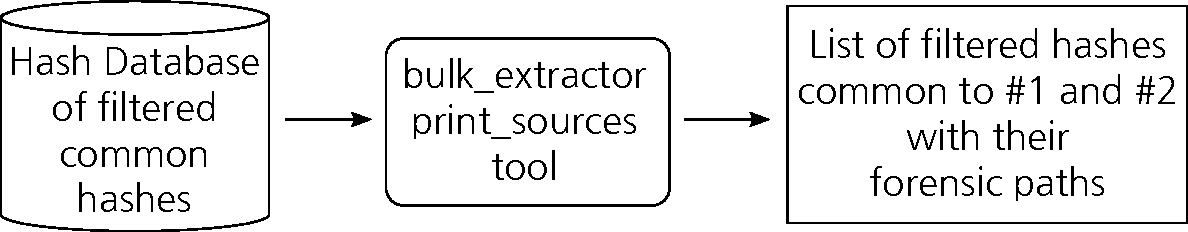
\includegraphics[scale=0.6]{drawings/import}
  \caption*{Run the \hdb \texttt{import} command
            to import block hashes into the hash database.}
\end{figure}

%steps
In this demo, we create a mock ``blacklist'' hash database.
We use the \texttt{demo\_video.mp4} file referenced in the scanner demo,
so the resultant \texttt{demo\_video\_db} hash database in this demo
is the same as the database used in that demo.
Here are the steps to perform this demo:
\begin{compactenum}
\item Download and install \hdb  and \bulk compiled with the \hashid scanner
from
\url{http://digitalcorpora.org/downloads/hashdb}
as described in the Scanner demo
for finding part of a video file in a media image,
\url{http://digitalcorpora.org/downloads/hashdb/demo/scanner\_demo.pdf}
\item Pick an file or directory to use
as your source of whitelist or blacklist files.
For this demo, please download file
\url{http://digitalcorpora.org/downloads/hashdb/demo/demo\_video.mp4}.

\item Use the \mdd tool to generate the DFXML file of block hashes
of your files and directories:
\begin{compactitem}
\item Use \texttt{-p 4096} to specify a block (partition) size of 4096.
\item Use \texttt{-d} to generate output in DFXML format.
\item If you are generating block hashes recursively in subdirectories,
rather than from a file, use the \texttt{-r} option.
In this demo, we generate block hashes from a file,
so we do not use this option.
\item Use \texttt{> demo\_video\_dfxml} to direct the DFXML output
to go to file \texttt{demo\_video\_dfxml}.
\end{compactitem}
\begin{verbatim}
$ md5deep -p 4096 -d demo_video.mp4 > demo_video_dfxml
\end{verbatim}

\item Use the \hdb tool to \texttt{create} a new hash database
called \texttt{demo\_video\_db}:
\begin{verbatim}
$ hashdb create demo_video_db
\end{verbatim}

\item Use the \hdb tool to \texttt{import} the block hashes
from the DFXML file into the new hash database:
\begin{verbatim}
$ hashdb import demo_video_dfxml demo_video_db
\end{verbatim}
\end{compactenum}

This completes the demo.

\end{document}

